\documentclass[12pt, letterpaper]{article}
\usepackage[titletoc,title]{appendix}
\usepackage{color}
\usepackage{booktabs}
\usepackage[usenames,dvipsnames,svgnames,table]{xcolor}
\definecolor{dark-red}{rgb}{0.75,0.10,0.10}
\definecolor{bluish}{rgb}{0.05,0.05,0.85}
\PassOptionsToPackage{unicode}{hyperref}
\PassOptionsToPackage{naturalnames}{hyperref}
\usepackage[margin=1in]{geometry}
\usepackage[linkcolor=blue,
			colorlinks=true,
			urlcolor=blue,
			pdfstartview={XYZ null null 1.00},
			pdfpagemode=UseNone,
			citecolor={bluish},
			pdftitle={partisan adult}]{hyperref}

%\newcites{SI}{SI References}
\usepackage{natbib}

\usepackage{float}
\usepackage{placeins}

\usepackage{geometry}  % see geometry.pdf on how to lay out the page. There's lots.
\geometry{letterpaper} % This is 8.5x11 paper. Options are a4paper or a5paper or other...
\usepackage{graphicx}  % Handles inclusion of major graphics formats and allows use of
\usepackage{amsfonts,amssymb,amsbsy}
\usepackage{amsxtra}
\usepackage{verbatim}
%\setcitestyle{round,semicolon,aysep={},yysep={;}}
\usepackage{setspace} % Permits line spacing control. Options are:
%\doublespacing
%\onehalfspace
%\usepackage{sectsty}    % Permits control of section header styles
\usepackage{pdflscape}
\usepackage{fancyhdr}   % Permits header customization. See header section below.
\usepackage{url}        % Correctly formats URLs with the \url{} tag
\usepackage{fullpage}   %1-inch margins
\usepackage{multirow}
\usepackage{verbatim}
\usepackage{rotating}
\setlength{\parindent}{3em}

%\usepackage[T1]{fontenc}
%\usepackage[bitstream-charter]{mathdesign}

\usepackage{chngcntr}
\usepackage{longtable}
\usepackage{adjustbox}
\usepackage{dcolumn}

\usepackage[nameinlink, capitalize, noabbrev]{cleveref}

\def\citeapos#1{\citeauthor{#1}'s (\citeyear{#1})}

\makeatother

\usepackage{footmisc}
\setlength{\footnotesep}{\baselineskip}
\makeatother
\renewcommand{\footnotelayout}{\normalsize \doublespacing}


% Colors
\usepackage{color}

\newcommand{\bch}{\color{blue}\em  }   % begin change
\newcommand{\ying} {\color{orange}\em  }   % begin change
\newcommand{\bgcd} {\color{purple}\em }
\newcommand{\ech}{\color{black}\rm  }    % end change

% Caption
\usepackage[hang, font=small,skip=0pt, labelfont={bf}]{caption}
%\captionsetup[subtable]{font=small,skip=0pt}
\usepackage{subcaption}

% tt font issues
% \renewcommand*{\ttdefault}{qcr}
\renewcommand{\ttdefault}{pcr}




\usepackage{lscape}
\renewcommand{\textfraction}{0}
\renewcommand{\topfraction}{0.95}
\renewcommand{\bottomfraction}{0.95}
\renewcommand{\floatpagefraction}{0.40}
\setcounter{totalnumber}{5}
\makeatletter
\providecommand\phantomcaption{\caption@refstepcounter\@captype}
\makeatother


\title{\Large{Holier Than Thou? No Partisan Gap in the Consumption\\ of Pornography Online}\footnote{You can download the replication materials from \href{http://github.com/soodoku/adult}{https://github.com/soodoku/adult}}}

\author{Lucas Shen\thanks{Lucas is a Research Fellow at Asia Competitiveness Institute, Lee Kuan Yew School of Public Policy, at the National University of Singapore, \href{mailto:lucas@lucasshen.com}{\footnotesize{\texttt{lucas@lucasshen.com}}}} \and Gaurav Sood\thanks{Gaurav can be reached at \href{mailto:gsood07@gmail.com}{\footnotesize{\texttt{gsood07@gmail.com}}}}\vspace{.5cm}}

\date{\today}

\begin{document}
\maketitle

\begin{comment}

setwd("~/Documents/Github/adult/ms/")
tools::texi2dvi("adult.tex", pdf=TRUE, clean=TRUE) 

\end{comment}

\thispagestyle{empty}
\begin{abstract}
\noindent Consumption of pornography has been blamed for a variety of societal ills, including the rise in misogyny, sex crimes, and the coarsening of culture. Using passively collected browsing data from YouGov, we investigate how much pornography Americans consume online. We find that there is a sharp positive skew in the consumption of pornography, with a small number of users consuming lots of pornography and most consuming small amounts. Only about 32 percent of the respondents consumed pornography online during the month long observation period. Of the people who consumed pornography, the median consumer spent about 44 minutes  consuming pornography and 95 percent spent less than 337 minutes. Lastly, we find that, unlike previous research \citep{macinnis2015american, edelman2009markets}, which relied on ecological inference, Democrats consume about as much pornography online as Republicans.
\end{abstract} 
\clearpage
\setcounter{page}{1}
\doublespace

Consumption of pornography is associated with a variety of disturbing attitudes, beliefs, emotions, and behaviors. Consuming pornography is associated with support for violence against women \citep{hald2010pornography, malamuth2012pornography, donnerstein1984pornography}, belief in rape myths \citep{foubert2011pornography}, increased gender role conflict, lesser sexual satisfaction \citep{szymanski2014psychological, stewart2012young}, poorer relationship quality \citep{szymanski2014psychological, szymanski2015male}, and sexually risky behaviors such as engaging in paid sex, and having extramarital sex \citep{wright2012internet}. A lot of popular pornography also contains a healthy dose of violence. An analysis of popular pornography revealed that 88.2\% of the scenes contained physical aggression, and 48.7\% verbal aggression \citep{bridges2010aggression}. For all these reasons, there are serious concerns about consumption of pornography.

In this paper, we investigate how much pornography Americans consume online. Using passive browsing data from YouGov, we find that there is a sharp skew in the consumption of pornography, with a small set of users consuming a large chunk of pornography. About 68 percent of the respondents abstained from consuming pornography online during the month long observation period. Of the people who consumed pornography, the median consumer spent about 44 minutes consuming pornography and the 95th percentile consumer spent 337 minutes. 

We also use the data to shed light on an age-old debate---whether Democrats consume more pornography than Republicans or vice versa. Both parties claim the higher moral ground. And in surveys both parties think consumption of pornography is abhorrent. Unlike previous research, which relied on ecological inference, we find that Democrats consume about as much pornography online as Republicans \citep{macinnis2015american, edelman2009markets}. Adjusting for background attributes like age, gender etc., makes little difference.

\section*{Data}\label{sec:data}
We use data from YouGov to measure the consumption of adult content \citep{data-dataverse}. YouGov maintains a large panel that is recruits using various methods. YouGov uses matched sampling to survey respondents: it first draws a random sample from a large synthetic representative sampling frame, finds respondents that match the sampled individuals from its panel, and invites them to take a survey. For data on how well Yougov is able to approximate a random sample, see \citet{rivers2009}. For our sample, panelists also shared de-identified web browsing data tracked via passive metering software installed voluntarily on their computers. The software, called RealityMine, captures online visits independent of the type of browser or browser-specific privacy settings.

The data are from 1,200 respondents and contains a month of data from June, 2022. In all, we have data on about 6 million visits. For each visit, we have information on the domain (e.g., wikipedia.org), the time of visit, and the time spent on the domain. The respondents visited about 64k unique sites, of which 900 are pornographic sites. 

Our data also includes characteristics of the 1,200 individuals. We have data on demographic characteristics like birth year, state, gender, race, and education level. We also have information on their party identification. Except for 120 respondents  who did not respond or picked not sure/don't know, the rest stated the party they identified with.  Of the 1,080 individuals who report party identification, 82 percent lean either Republican or Democrat. The remaining 18 percent identify as independent. 

\section*{Measuring Pornographic Content}
We code pornographic content at the domain level. Our main analysis depends on the domain classifications that come with YouGov data. We code domains that YouGov categorizes as ``Adult'' as pornographic sites. These include ``Adult'' (e.g., xvideos.com), ``Adult, Business'' (e.g., onlyfans.com), and ``Adult, Entertainment'' (e.g., hentainfox.com). Yougoc classifies certain domains as 'Adult' that do not primarily carry pornographic content, e.g., urbandictionary.com and 4chan.org . Given the skew in the data (See \cref{fig:top25_adult} and \cref{fig:top25_nonadult})\footnote{We use the \texttt{forestplot} \citep{forestplot} and \texttt{tableone} \citep{tableone} packages to tabulate key descriptive figures.}, we manually check the top adult domains to remove such sites. If there is graphic nudity on the landing page or if the site is some form of erotica, we classify the site as a pornographic. 

In \ref{si:alternate_ways}, we leverage the \texttt{piedomains} package to classify which domains are pornographic sites using machine learning \citep{Chintalapati_piedomains_Predict_the_2022}. We leverage the probability estimates to produce a low false negative and low false positive version. The key results remain unchanged. 


\section*{Results}

\subsection*{Consumption of Pornography}
Across all respondents, only a small fraction of the web browsing visits, approximately 84,000 visits or 1.3 percent, are to pornographic sites. And these visits are concentrated among a few people. Only about 32 percent of the respondents consumed pornography online during the sample period. The average consumer of pornography online spent approximately 230 minutes (standard deviation of 576 minutes). 

The consumption of pornography is also highly concentrated among a few sites, with ten most frequented pornography sites receiving more than 12 times the traffic to all other pornographic sites  (approximately 109 minutes vs. 9 minutes, see \cref{fig:concentration_porn_consumption}). Close to 80 percent of the traffic to pornographic sites is to just one pornographic site. Looking at the characteristics of consumers of pornography, expectedly, consumers of pornography online are younger and are more likely to be male \cref{fig:} %TODO

\subsection*{Partisan Differences in Consumption of Pornography Online}
Our primary dependent variables of interest are: total time spent on pornographic sites and the proportion of time spent on pornographic sites. (In \ref{si:visits}, we show similar analysis for visits. The upshot is that the key conclusions are unaffected.)

Given the skew in the data, we ran a quantile regression, regressing the duration on party. As Figures \ref{fig:quantile_regression_duration} and \ref{fig:quantile_regression_prop_duration} show, there are no significant differences in consumption of pornographic content between the parties. To account for the possibility that this may be a result of confounding demographic differences between the parties, we control for immutable characteristics like age and gender. (\cref{tab:characteristics_split_by_party} shows differences in age, gender, and race by party identification.) We use these variables in our analyses of pornography consumption below. Given how concentrated pornographic consumption is in our data, it is unlikely to make much of a difference and that is indeed what we find --- see Figure \ref{fig:quantile_regression_duration}. 
%===========================
% Quantile regressions
% Hours spent on adult sites
%===========================
\begin{figure}[t]
	\centering
	\caption{Quantile Estimates--Hours Spent on Pornographic Sites by Party}
	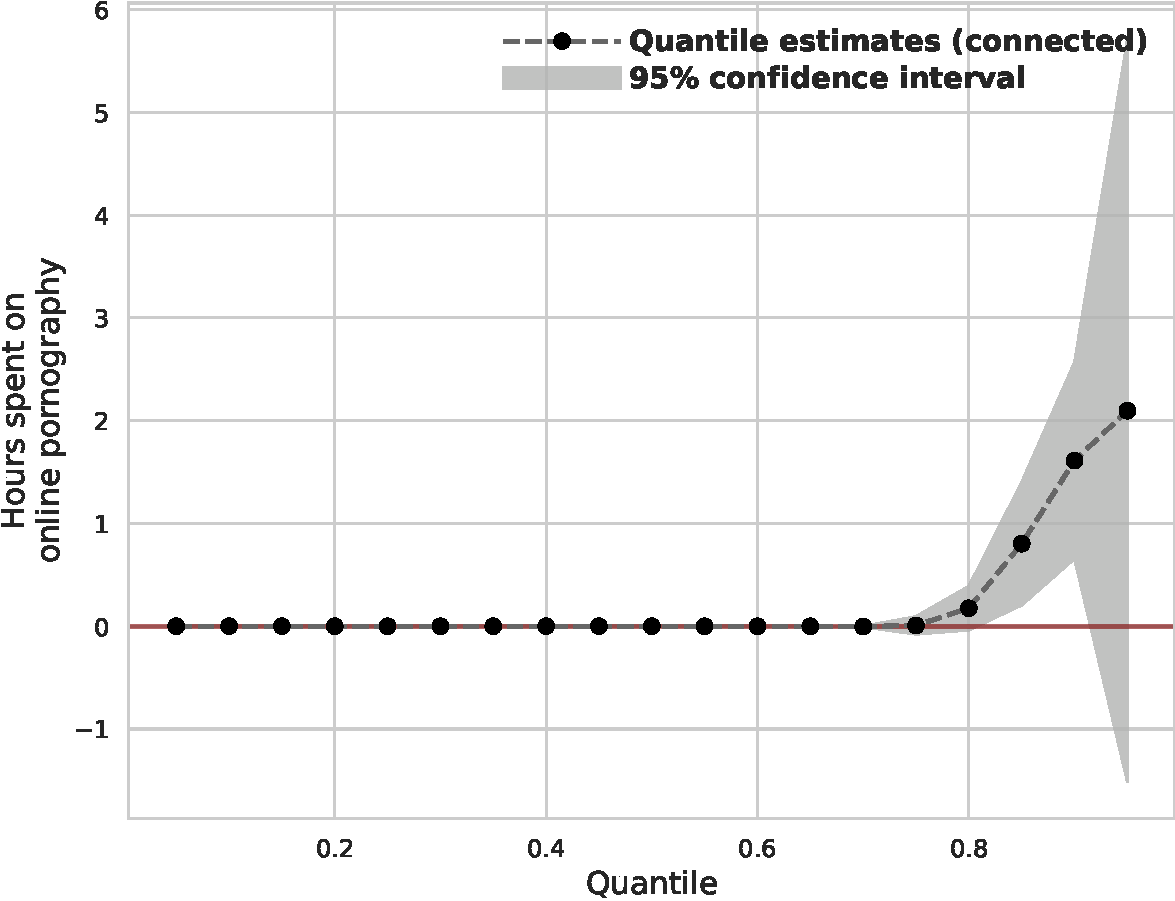
\includegraphics[width=.7\linewidth]{../figs/quantile_reg_duration_adult.pdf}
	\caption*{\footnotesize \emph{Notes:} 
		Dependent variable is the number of hours individuals in our sample spent on pornographic sites.
		Each point indicates the difference between Republicans and Democrats and corresponds to a quantile regression at the quantile indicated by the x-axis.
		95\% confidence intervals constructed from standard errors.
		See \cref{fig:quantile_regression_duration_covariates} for the same plot controlling for individual characteristics.
	}
	\label{fig:quantile_regression_duration}
\end{figure}

%========================================
% Quantile regressions
% Proportion of time spent on adult sites
%========================================
\begin{figure}[t]
	\centering
	\caption{Quantile Estimates--Percentage of Time Spent on Pornographic Sites by Party}
	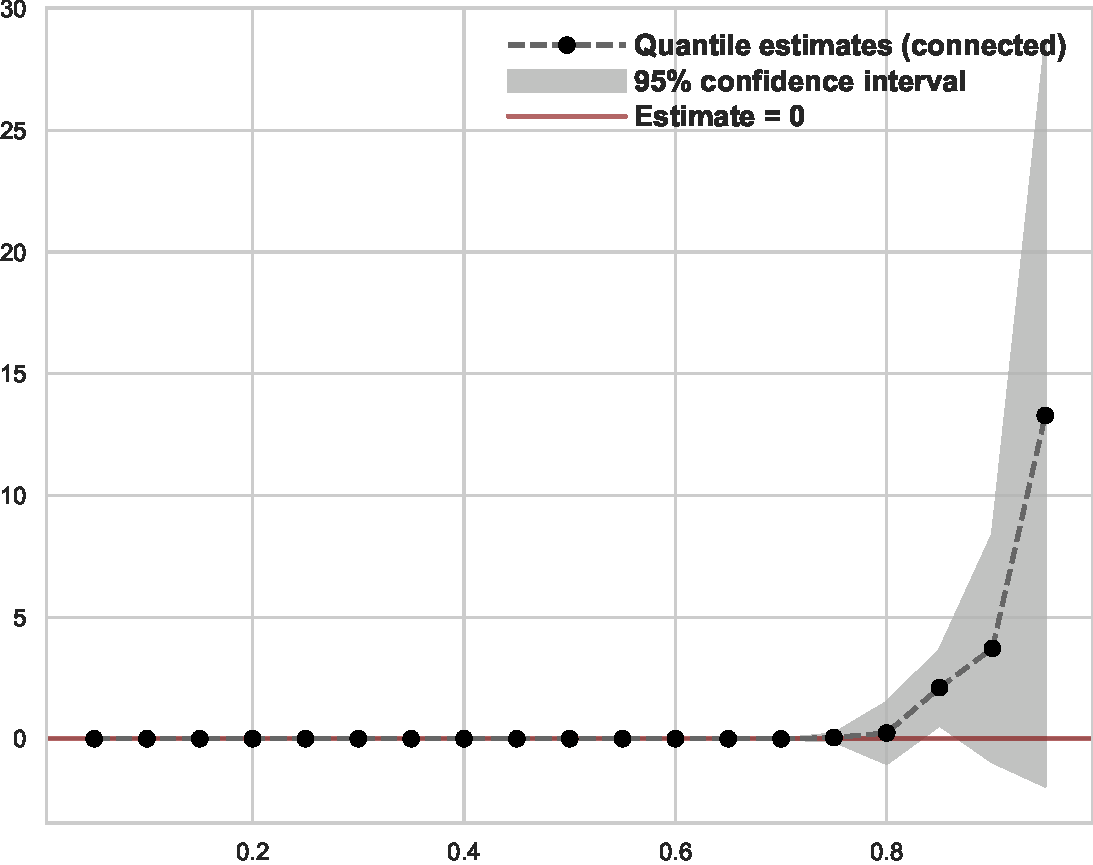
\includegraphics[width=.7\linewidth]{../figs/quantile_reg_proportion_duration_adult.pdf}
	\caption*{\footnotesize \emph{Notes:} 
		Dependent variable is the percentage of time individuals in our sample spent on pornographic sites.
		Each point indicates the difference between Republicans and Democrats and corresponds to a quantile regression at the quantile indicated by the x-axis.
		95\% confidence intervals constructed from standard errors.
		See \cref{fig:quantile_regression_prop_duration_covariates} for the same plot controlling for individual characteristics.
	}
	\label{fig:quantile_regression_prop_duration}
\end{figure}


\section*{Discussion}

Consumption of pornography has been attributed to a variety of ills. It is also considered problematic from a religious perspective. For instance, Christian theologians believe that consumption of pornography leads people away from purity and hence should be avoided.\footnote{\url{https://www.churchofjesuschrist.org/study/manual/help-for-pornography-users/effect-of-pornography}}. The Internet has dramatically increased access to pornography. This has led to the concern that pornography consumption has become very widespread and extensive. Our data suggest that pornography consumption online is highly concentrated with very few people consuming a lot of pornography and most people consuming very little or none.

The second contribution of our paper is estimates of partisan differences in consumption of pornography online. Both the parties claim the higher ground when it comes to women---one's case for morality is steeped in religion, the other's in enduring concern for women. Our data suggest that the partisan differences are likely very small.

Our research has three major limitations. The first concern with our data is that we may not have all the Internet visitation data from a user. If the respondent changes their behavior in response to the knowledge that their data is being collected (even if it is de-identified), for e.g., they may modify their behavior on the machine or figure out ways to evade detection, it may bias our results. In fact, we think it is likely that people would be less likely to search for pornography on machines on which they have installed passive monitoring software (though the data are de-identified). If that is so, our estimates are a lower bound of net consumption of pornography. If this bias varies by party, our estimates of partisan differences will also be biased. 

The second concern with our measurement is that we code content at a domain level. This runs the risk of incurring some ecological fallacy. For instance, our classification would code websites like Tumblr as not carrying pornographic content but some of Tumblr content is pornographic. 

The third concern is that our measures are a point in time. We have data from one month in one year---June, 2022. It is possible that people consume less pornography online and instead spend time outside in June when the weather in many parts of the US is more pleasant than in preceding or following months. 

\clearpage
\bibliographystyle{apsr}
\bibliography{porn}
\clearpage

%===============================================================================
%===============================================================================
% Appendix
%===============================================================================
%===============================================================================
\appendix
\renewcommand{\thesection}{SI \arabic{section}}
\renewcommand\thetable{\thesection.\arabic{table}}  
\renewcommand\thefigure{\thesection.\arabic{figure}}
\counterwithin{figure}{section}
\counterwithin{table}{section}
\begin{center}
\Large{Supporting Information}
\end{center}

\FloatBarrier
%===============================================================================
% Supplementary Descriptives for sense of landscape of porn consumption
%===============================================================================
\section{Descriptive Analysis}

\subsection{Skew in Website Visits}
%============================
% Figure of top 25 adultsites
%============================
\begin{figure}[ht]
	\centering
	\caption{Top 25 Pornography Sites}
	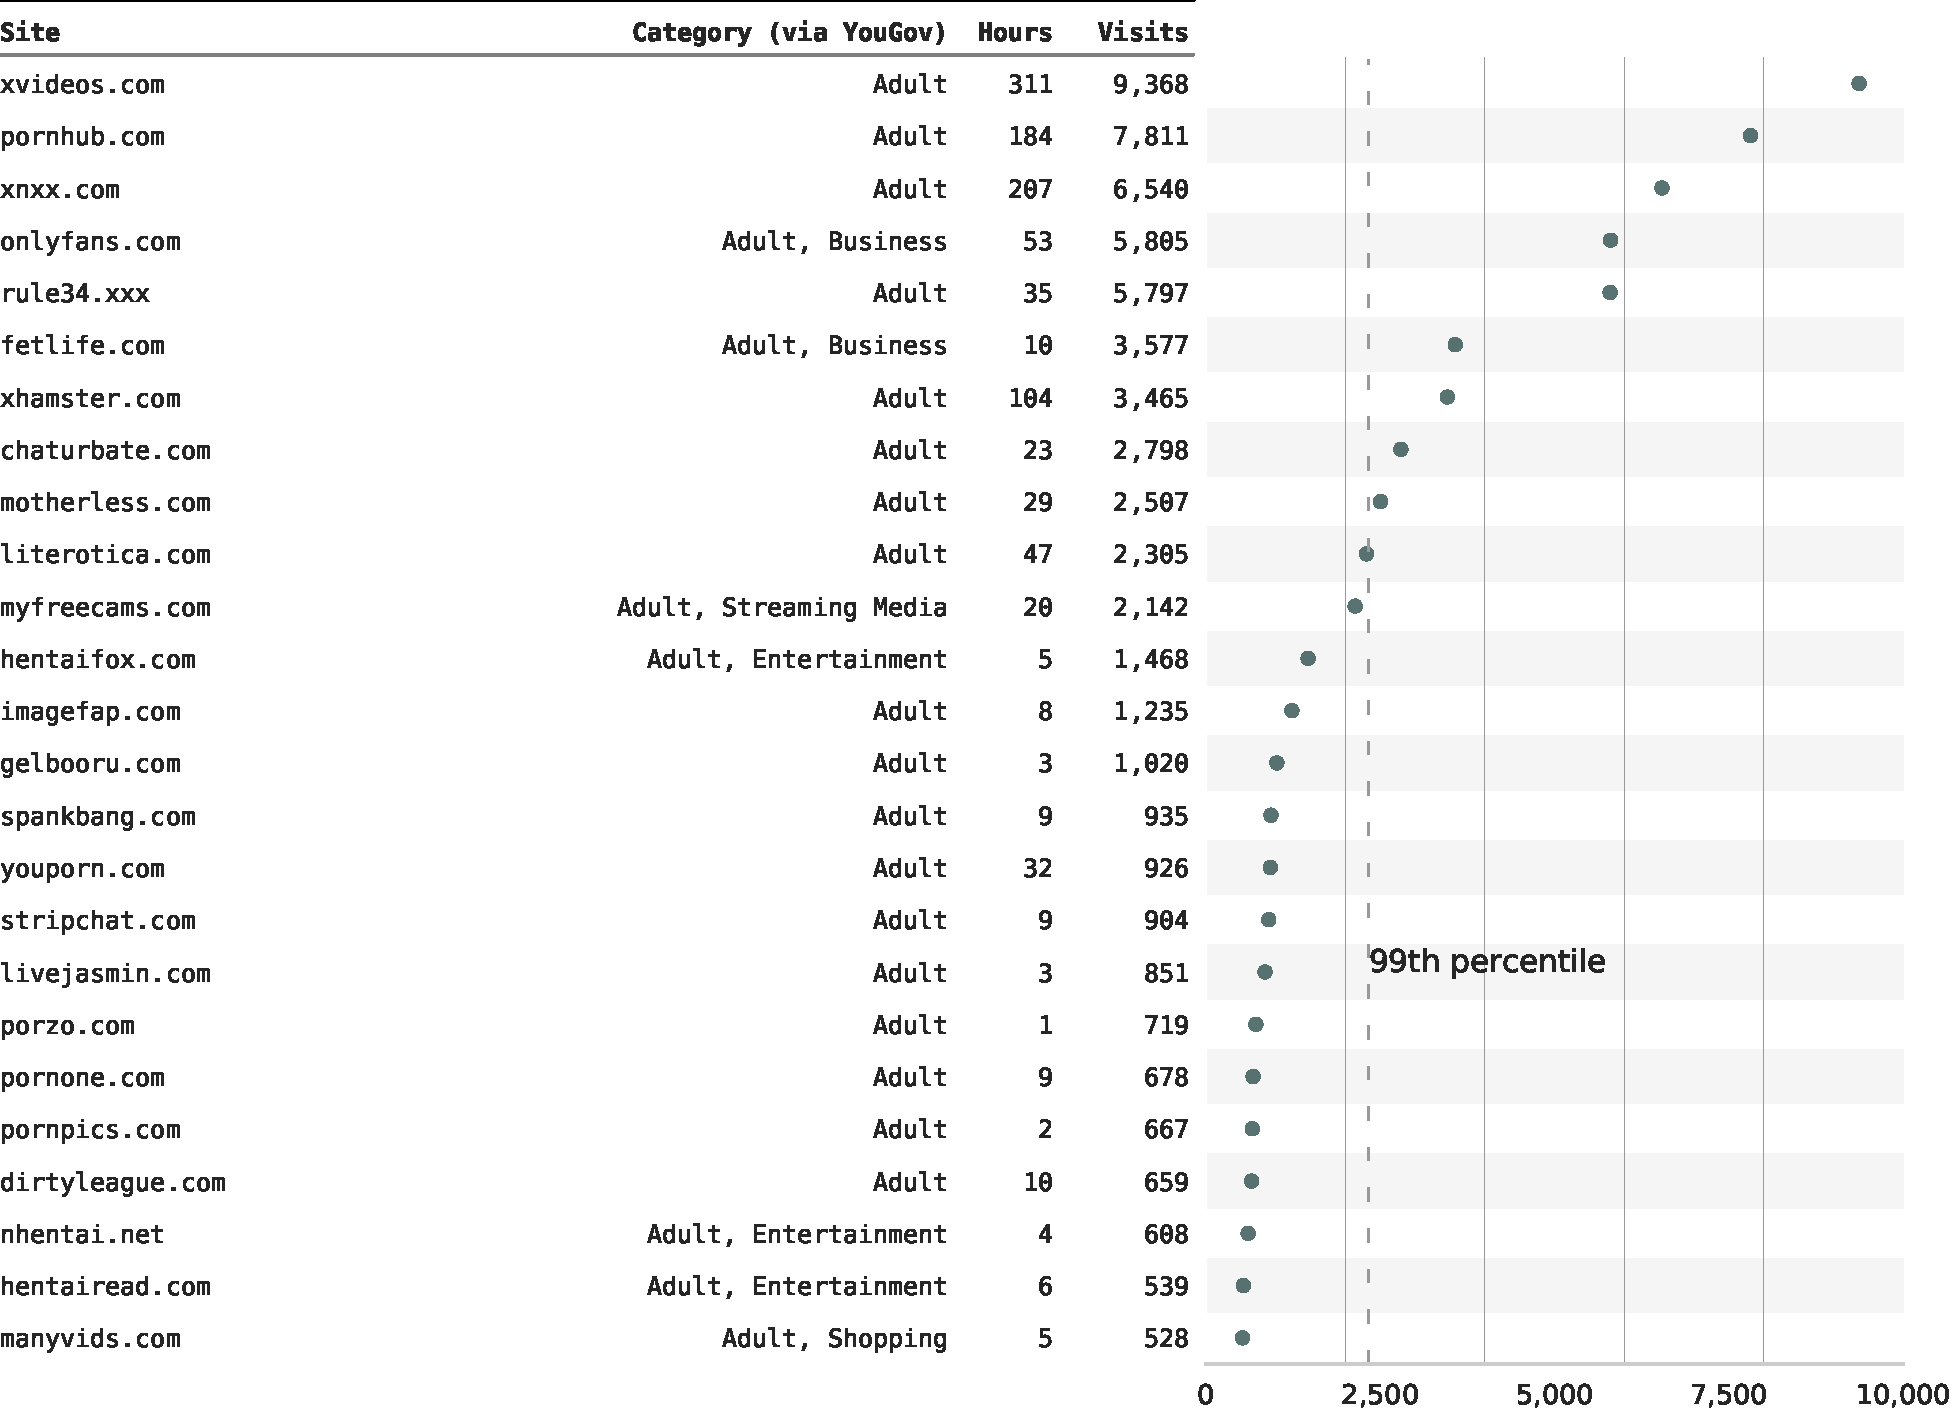
\includegraphics[width=\textwidth]{../figs/top_25_adultsites.pdf}
	\caption*{\footnotesize \emph{Notes:} 
		Table shows the top 25 pornographic sites that individuals visit in the sample period.
		Pornography sites are as categorized by YouGov (see the \nameref{sec:data} section).
		The \emph{Hours} column are the total number of hours that individuals in the sample spent on the site. 
		The \emph{Visits} column is total number of visits by individuals in the sample to the site.  
		Sites to the right of the vertical dashed are the top 1 percent of pornographic sites.
	}
	\label{fig:top25_adult}
\end{figure}

%================================
% Figure of top 25 non-adultsites
%================================
\begin{figure}
	\centering
	\caption{Top 25 (Non-Porn) Domains}
	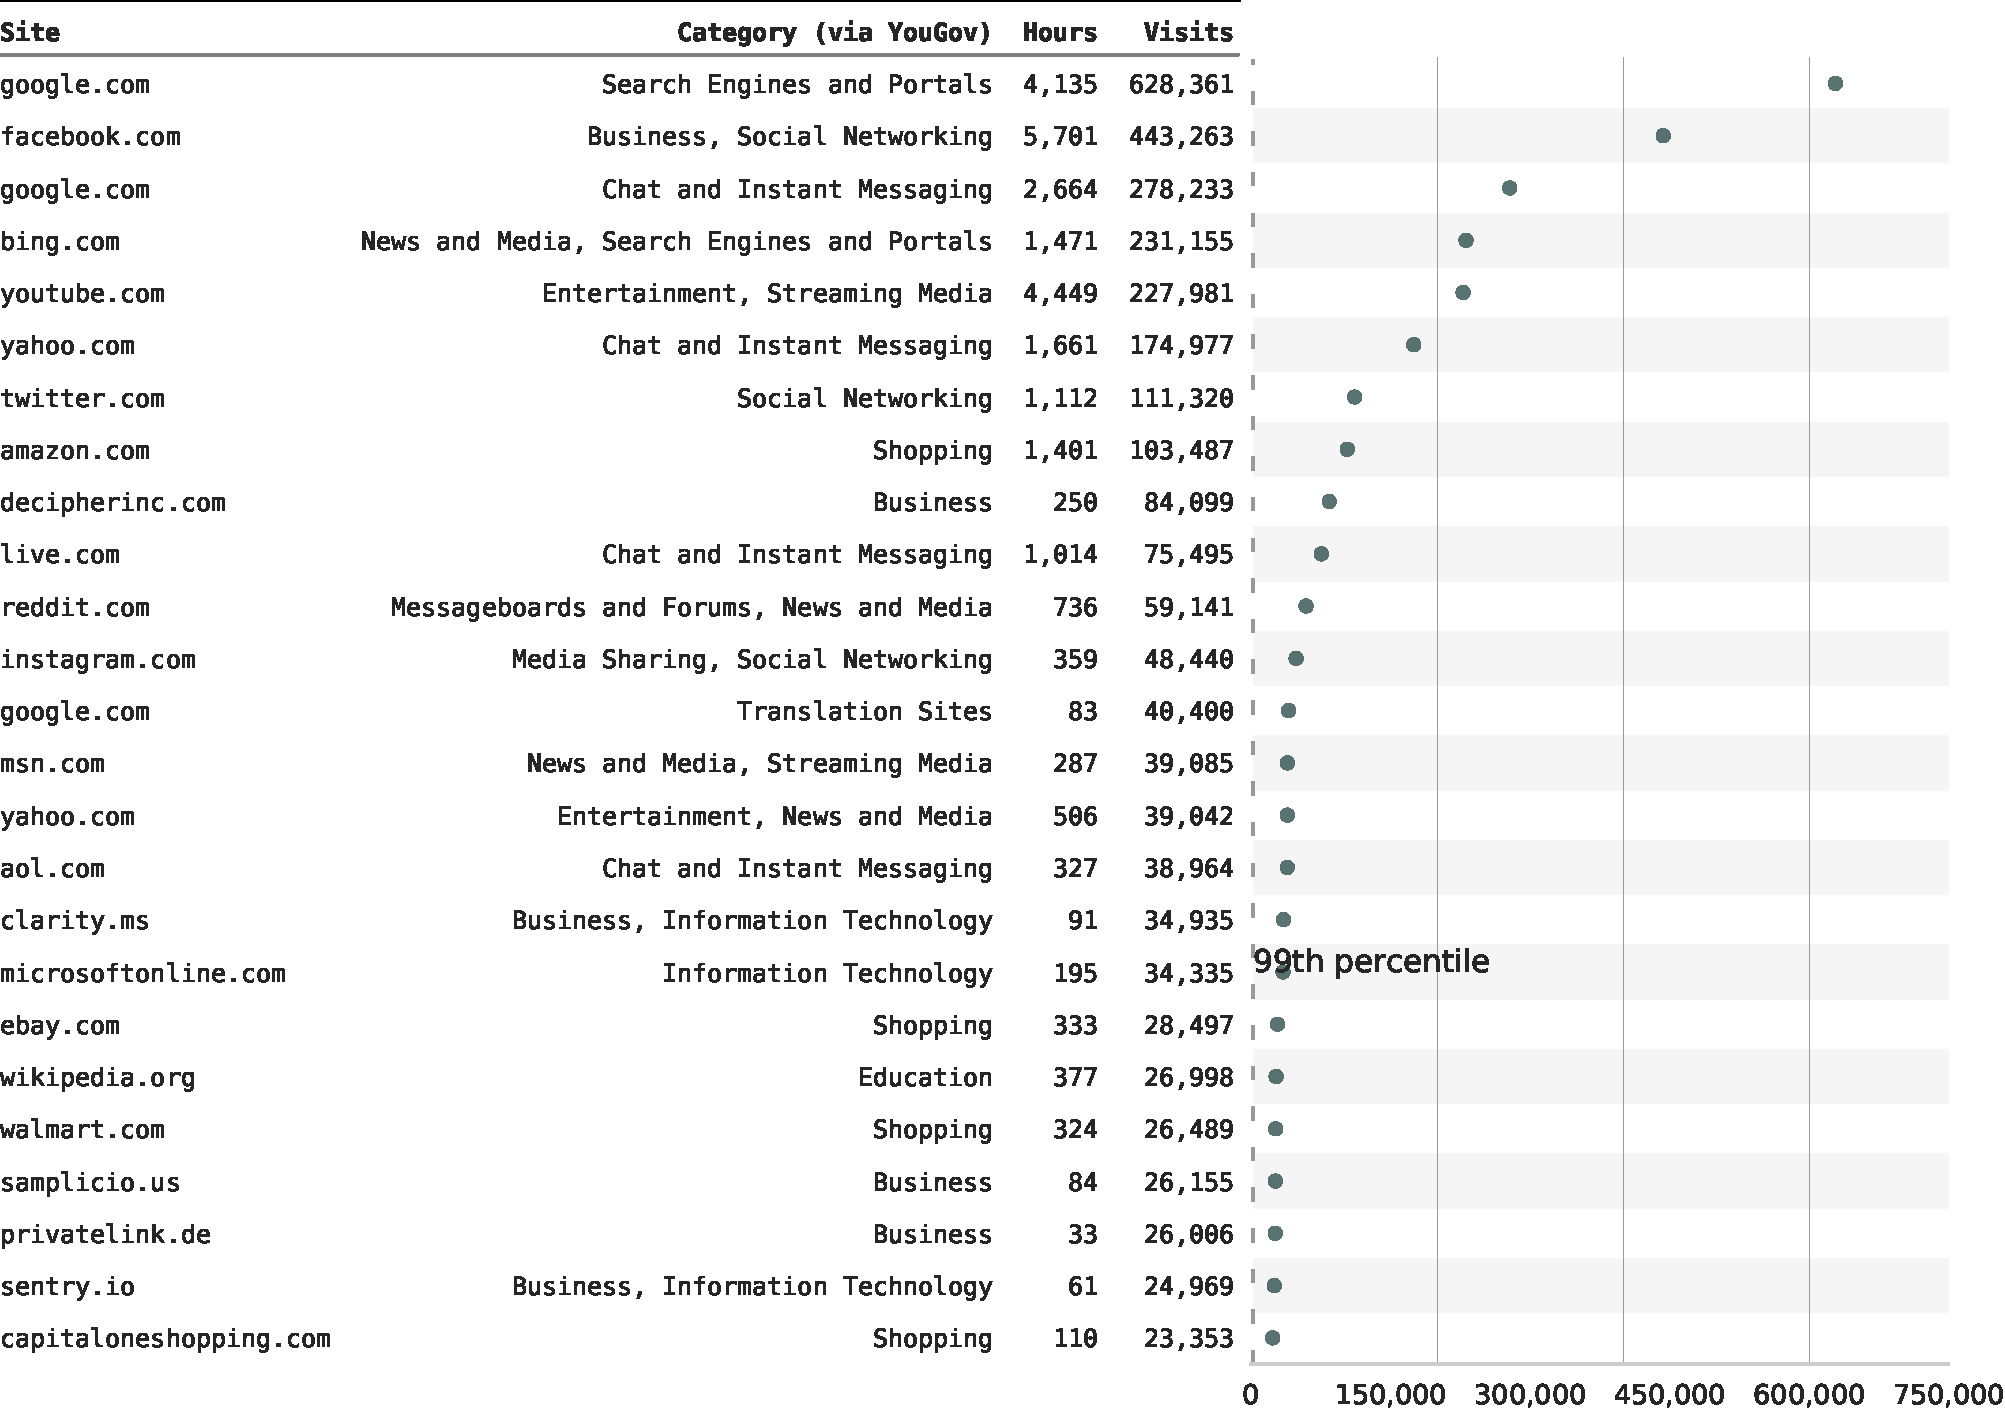
\includegraphics[width=\textwidth]{../figs/top_25_nonadultsites.pdf}
	\caption*{\footnotesize \emph{Notes:} 
		Table shows the top 25 non-pornographic sites that individuals visit in the sample period.
		The \emph{Hours} column are the total number of hours that individuals in the sample spent on the site. 
		The \emph{Visits} column is total number of visits by individuals in the sample to the site.  			
		Sites to the right of the vertical dashed are the top 1 percent (of non-pornographic sites).
	}
	\label{fig:top25_nonadult}
\end{figure}


%=============================================
% Figure for concentration of porn consumption
%=============================================
\begin{figure}
	\centering
	\caption{Traffic to Top 10 Pornographic Sites}
	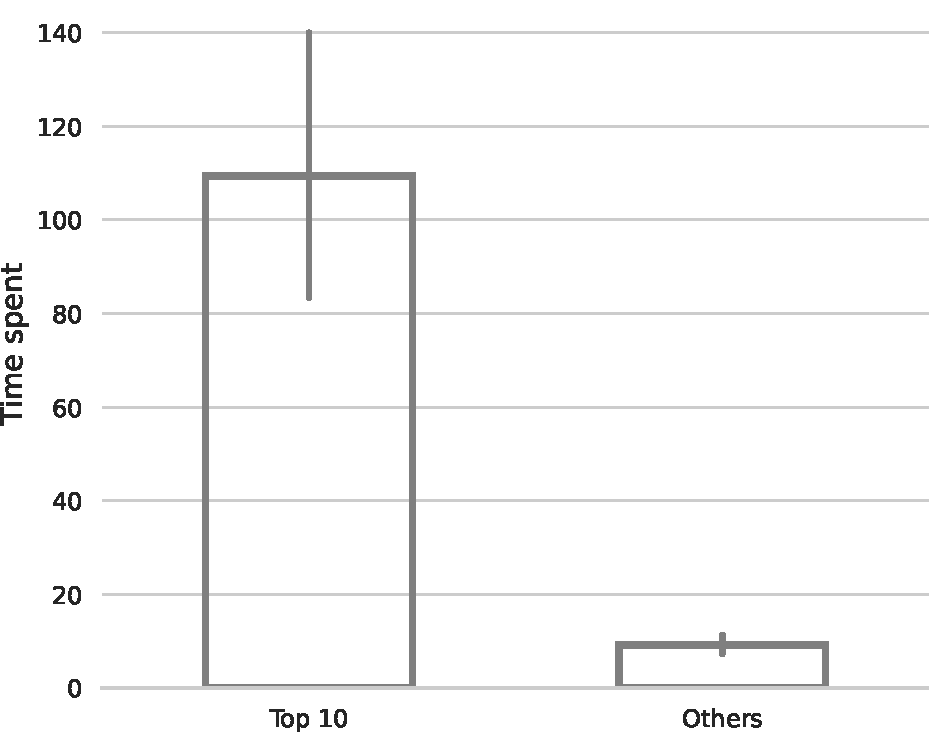
\includegraphics[width=.5\textwidth]{../figs/concentration_porn_consumption.pdf}
	\caption*{\footnotesize \emph{Notes:} 
		The Top 10 bar indicates traffic to the top 10 pornographic sites in the data (see \cref{fig:top25_adult}).
		The Others bar indicates traffic to all other pornographic sites outside of the top 10.
		The y-axis is the total time spent on pornographic sites, averaged across individuals.
		Time units is hours.
		Vertical bars are 95\% confidence intervals from bootstrapped standard errors (n = 1,000).
	}
	\label{fig:concentration_porn_consumption}
\end{figure}

%====================================
% Figure of traffic to top x websites
%====================================
\begin{figure}
	\centering
	\caption{Traffic to Top x Pornographic Sites by Party}
	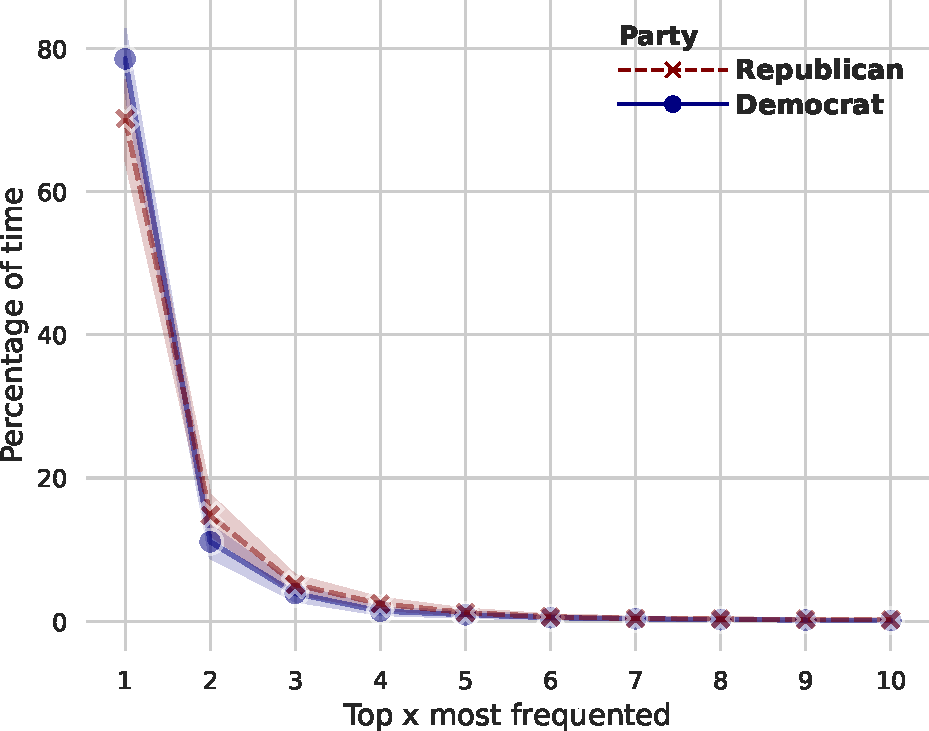
\includegraphics[width=.6\textwidth]{../figs/concentration_porn_consumption_topX_by_party.pdf}
	\caption*{\footnotesize \emph{Notes:} 
		Figure shows concentration of pornography consumption based on individuals' most frequented pornographic sites.
		Shaded areas are 95\% confidence intervals from bootstrapped standard errors (n = 1,000).
	}
	\label{fig:concentration_porn_consumption_topX_by_party}
\end{figure}


\FloatBarrier
\subsection{Skew in Consumption of Pornographic Content}
%====================================================
% Tabulated percentiles of hours spent on adult sites
%====================================================
\begin{table}[ht] \centering \small \setlength\tabcolsep{10 pt}
	\caption{Distribution of Consumption of Pornography Online}
	\label{tab:distribution_duration}
	\begin{adjustbox}{max width=\textwidth}
		\begin{tabular}{cr}
			\toprule
			\multicolumn{1}{c}{\textbf{Percentile}}&\multicolumn{1}{c}{\textbf{Hours}}\\
			\midrule
			0.00 &  0.00 \\
0.10 &  0.02 \\
0.20 &  0.07 \\
0.30 &  0.16 \\
0.40 &  0.33 \\
0.50 &  0.64 \\
0.60 &  1.30 \\
0.70 &  2.20 \\
0.80 &  4.49 \\
0.90 & 10.15 \\
0.95 & 19.50 \\
0.96 & 21.93 \\
0.97 & 27.31 \\
0.98 & 32.22 \\
0.99 & 46.47 \\
1.00 & 93.96 \\\\
			\bottomrule
		\end{tabular}
	\end{adjustbox}
	\caption*{\footnotesize \emph{Notes:} 
		Table shows key percentiles (each of the ten deciles plus quantiles at the right tail) and their corresponding values for the duration (hours) spent by individuals who consumed pornography in the sample period. 
		%See \cref{fig:distribution_duration} for the plot.
	}
\end{table}

%=====================================================================
% Tabulated percentiles of proportion of duration spent on adult sites
%=====================================================================
\begin{table}[ht] \centering \small \setlength\tabcolsep{10 pt}
	\caption{Percentage of Time Spent on Pornographic Sites}
	\label{tab:distribution_prop_duration}
	\begin{adjustbox}{max width=\textwidth}
		\begin{tabular}{cr}
			\toprule
			\multicolumn{1}{c}{\textbf{Percentile}}&\multicolumn{1}{c}{\textbf{\% time}}\\
			\midrule
			0.00 &  0.0 \\
0.10 &  0.0 \\
0.20 &  0.1 \\
0.30 &  0.5 \\
0.40 &  1.0 \\
0.50 &  2.4 \\
0.60 &  4.3 \\
0.70 &  7.9 \\
0.80 & 13.5 \\
0.90 & 34.3 \\
0.95 & 55.6 \\
0.96 & 62.8 \\
0.97 & 64.3 \\
0.98 & 68.9 \\
0.99 & 73.9 \\
1.00 & 87.5 \\
			\bottomrule
		\end{tabular}
	\end{adjustbox}
	\caption*{\footnotesize \emph{Notes:} 
		Table shows key percentiles (each of the ten deciles plus quantiles at the right tail) and their corresponding values for the duration (hours) spent by individuals who consumed pornography in the sample period. 
		%See \cref{fig:distribution_prop_duration} for the plot.
	}
\end{table}

\FloatBarrier
\section{Partisan Differences}
\subsection{Distribution of Differences}
%===========================================================================
% Tabulated splits by party and by percentiles for hours spent on adultsites
%===========================================================================
\begin{table}[ht] \centering \small \setlength\tabcolsep{10 pt}
	\caption{Distribution of Consumption of Pornography Online by Party}
	\label{tab:distribution_duration_party}
	\begin{adjustbox}{max width=\textwidth}
		\begin{tabular}{crr}
			\toprule
			\multicolumn{1}{l}{\textbf{}}&\multicolumn{2}{c}{\textbf{Hours}}\\
			\cmidrule(l){2-3}
			\multicolumn{1}{l}{\textbf{Percentile}}&\multicolumn{1}{c}{\textbf{Republicans}}&\multicolumn{1}{c}{\textbf{Democrats}}\\
			\midrule
			0.00 &  0.00 &  0.00 \\
0.10 &  0.04 &  0.02 \\
0.20 &  0.12 &  0.05 \\
0.30 &  0.29 &  0.11 \\
0.40 &  0.58 &  0.18 \\
0.50 &  1.36 &  0.38 \\
0.60 &  2.11 &  0.69 \\
0.70 &  3.04 &  1.37 \\
0.80 &  5.51 &  3.41 \\
0.90 & 11.57 &  7.15 \\
0.95 & 24.91 & 15.57 \\
0.96 & 26.91 & 17.33 \\
0.97 & 27.74 & 19.28 \\
0.98 & 29.30 & 21.65 \\
0.99 & 36.59 & 43.01 \\
1.00 & 37.54 & 90.48 \\\\
			\bottomrule
		\end{tabular}
	\end{adjustbox}
	\caption*{\footnotesize \emph{Notes:} 
		Table shows splits by party and by key percentiles (each of the ten deciles plus quantiles at the right tail) for the duration (hours) spent by individuals who consumed pornography in the sample period. 
		%See \cref{fig:distribution_duration_party} for the plot.
	}
\end{table}

%===============================================================================
% Tabulated splits by party and by percentiles for proportion of time spent on adultsites
%===============================================================================
\begin{table}[ht] \centering \small \setlength\tabcolsep{10 pt}
	\caption{Percentage of Time Spent on Pornographic Sites by Party}
	\label{tab:distribution_prop_duration_party}
	\begin{adjustbox}{max width=\textwidth}
		\begin{tabular}{crr}
			\toprule
			\multicolumn{1}{l}{\textbf{}}&\multicolumn{2}{c}{\textbf{\% time}}\\
			\cmidrule(l){2-3}
			\multicolumn{1}{l}{\textbf{Percentile}}&\multicolumn{1}{c}{\textbf{Republicans}}&\multicolumn{1}{c}{\textbf{Democrats}}\\
			\midrule
			0.00 &  0.0 &  0.0 \\
0.10 &  0.0 &  0.0 \\
0.20 &  0.3 &  0.1 \\
0.30 &  0.8 &  0.2 \\
0.40 &  2.0 &  0.8 \\
0.50 &  3.8 &  1.3 \\
0.60 &  6.4 &  2.6 \\
0.70 & 10.6 &  5.6 \\
0.80 & 20.3 & 11.4 \\
0.90 & 36.3 & 33.3 \\
0.95 & 44.2 & 54.1 \\
0.96 & 52.9 & 56.6 \\
0.97 & 62.3 & 63.4 \\
0.98 & 68.4 & 64.9 \\
0.99 & 71.0 & 72.1 \\
1.00 & 87.5 & 77.4 \\\\
			\bottomrule
		\end{tabular}
	\end{adjustbox}
	\caption*{\footnotesize \emph{Notes:} 
		Table shows splits by party and by key percentiles (each of the ten deciles plus quantiles at the right tail) for the duration (hours) spent by individuals who consumed pornography in the sample period. 
		%See \cref{fig:distribution_prop_duration_party} for the plot.
	}
\end{table}

\FloatBarrier
\subsection{Accounting for Confounders}
%==============================================================================
% Table for balance of porn consumption and individual characteristics by party
%==============================================================================
\begin{table}[ht] \centering \small \setlength\tabcolsep{5 pt}
	\caption{Differences in Pornography Consumption and Individual Characteristics by Party}
	\label{tab:characteristics_split_by_party}
	\begin{adjustbox}{max width=\textwidth}
		\begin{tabular}{@{\hspace{0\tabcolsep}}llrcccrr@{\hspace{0\tabcolsep}}}
			\toprule
			&\multicolumn{7}{c}{\underline{Panel A. Measures of pornography consumption}}\\
			&\multicolumn{1}{l}{(1)}&\multicolumn{1}{c}{(2)}&\multicolumn{1}{c}{(3)}&\multicolumn{1}{c}{(4)}&\multicolumn{1}{c}{(5)}&\multicolumn{1}{c}{(6)}&\multicolumn{1}{r}{(7)}\\			
			&\multicolumn{1}{l}{Subgroups}&\multicolumn{1}{c}{NA}&\multicolumn{1}{c}{Total}&\multicolumn{1}{c}{Democrat}&\multicolumn{1}{c}{Republican}&\multicolumn{1}{c}{P-val}&\multicolumn{1}{r}{SMD}\\
			\cmidrule{2-8}
			 n                      &     &           & 1200         & 530          & 356          &           &                 \\
 Consume porn, n (\%)    & No  & 65        & 774 (68.2)   & 343 (68.5)   & 235 (70.6)   & 0.569     & 0.046           \\
                        & Yes &           & 361 (31.8)   & 158 (31.5)   & 98 (29.4)    &           &                 \\
 Minutes, mean (SD)     &     & 65        & 73.4 (342.1) & 58.8 (331.7) & 75.8 (277.4) & 0.423     & 0.056           \\
 \% of time, mean (SD)   &     & 65        & 3.4 (11.2)   & 2.9 (10.7)   & 3.5 (11.1)   & 0.486     & 0.049           \\
 Visits, mean (SD)      &     & 65        & 74.3 (328.9) & 59.9 (298.9) & 73.7 (271.1) & 0.489     & 0.048           \\
 \% of visits, mean (SD) &     & 65        & 2.2 (7.1)    & 1.7 (6.1)    & 2.3 (7.1)    & 0.238     & 0.085           \\
			%-------------------------------------------------------------------
			\cmidrule{2-8}
			&\multicolumn{7}{c}{\underline{Panel B. Individual characteristics}}\\
			&\multicolumn{1}{l}{(1)}&\multicolumn{1}{c}{(2)}&\multicolumn{1}{c}{(3)}&\multicolumn{1}{c}{(4)}&\multicolumn{1}{c}{(5)}&\multicolumn{1}{c}{(6)}&\multicolumn{1}{r}{(7)}\\			
			&\multicolumn{1}{l}{Subgroups}&\multicolumn{1}{c}{NA}&\multicolumn{1}{c}{Total}&\multicolumn{1}{c}{Democrat}&\multicolumn{1}{c}{Republican}&\multicolumn{1}{c}{P-val}&\multicolumn{1}{r}{SMD}\\
			\cmidrule{2-8}
			 n                          &               &           & 1200        & 530         & 356         &           &                 \\
 Party (7-point), mean (SD) &               & 120       & 3.6 (2.2)   & 1.7 (0.8)   & 6.3 (0.8)   & \ensuremath{<}0.001    & 5.670           \\
 2020 Pres. election, n (\%) & Other/No vote & 170       & 270 (26.2)  & 97 (20.2)   & 47 (14.1)   & \ensuremath{<}0.001    & 3.296           \\
                            & Vote Biden    &           & 419 (40.7)  & 369 (76.9)  & 8 (2.4)     &           &                 \\
                            & Vote Trump    &           & 341 (33.1)  & 14 (2.9)    & 278 (83.5)  &           &                 \\
 Age, mean (SD)             &               & 0         & 49.5 (18.1) & 48.7 (17.8) & 55.4 (18.0) & \ensuremath{<}0.001    & 0.373           \\
 Gender, n (\%)              & Female        & 0         & 635 (52.9)  & 312 (58.9)  & 174 (48.9)  & 0.004     & 0.201           \\
                            & Male          &           & 565 (47.1)  & 218 (41.1)  & 182 (51.1)  &           &                 \\
 Race, n (\%)                & Asian         & 0         & 49 (4.1)    & 31 (5.8)    & 6 (1.7)     & \ensuremath{<}0.001    & 0.747           \\
                            & Black         &           & 152 (12.7)  & 96 (18.1)   & 7 (2.0)     &           &                 \\
                            & Hispanic      &           & 176 (14.7)  & 87 (16.4)   & 35 (9.8)    &           &                 \\
                            & Others        &           & 61 (5.1)    & 29 (5.5)    & 9 (2.5)     &           &                 \\
                            & White         &           & 762 (63.5)  & 287 (54.2)  & 299 (84.0)  &           &                 \\
 Education, n (\%)           & College       & 0         & 525 (43.8)  & 258 (48.7)  & 158 (44.4)  & 0.625     & 0.091           \\
                            & HS            &           & 354 (29.5)  & 146 (27.5)  & 103 (28.9)  &           &                 \\
                            & No HS         &           & 73 (6.1)    & 24 (4.5)    & 17 (4.8)    &           &                 \\
                            & Some college  &           & 248 (20.7)  & 102 (19.2)  & 78 (21.9)   &           &                 \\
 Region, n (\%)              & Midwest       & 8         & 239 (20.1)  & 100 (19.0)  & 83 (23.4)   & 0.034     & 0.204           \\
                            & Northeast     &           & 210 (17.6)  & 103 (19.6)  & 50 (14.1)   &           &                 \\
                            & South         &           & 502 (42.1)  & 208 (39.6)  & 159 (44.8)  &           &                 \\
                            & West          &           & 241 (20.2)  & 114 (21.7)  & 63 (17.7)   &           &                 \\
			\bottomrule
		\end{tabular}
	\end{adjustbox}
	\caption*{\scriptsize \emph{Notes:}
		Table shows splits by party for pornography consumption and for individual characteristics for the 1,200 individuals.
		Party identification is based on a 7-point scale. We code 1--3 as ``Democrat'', 4 as ``Independent'', 5--7 as ``Republican''.
		Column (1) shows subgroups for categorical variables.
		Column (2) indicates the count of missing variables, if any.
		Columns (3)--(5) show means and standard deviations for continuous variables and count and percentage of data for categorical variables, for the full sample, Democratic individuals, and Republican individuals.
		Standard deviations and percentages in parentheses.
		Column (6) and column (7) report the p-values and standardized mean differences for Democrats vs Republicans.
		Given the skew in consumption of pornography, we also performed tests for difference in means for the measures of pornography consumption by party. See \cref{tab:characteristics_split_by_party_medians}.
	}
\end{table}

%==============================================================================
% Table for balance of porn consumption and individual characteristics by party
%==============================================================================
\begin{table}[ht] \centering \small \setlength\tabcolsep{5 pt}
	\caption{Differences in Pornography Consumption and Individual Characteristics by Pornography Consumers}
	\label{tab:characteristics_split_by_porn_consumers}
	\begin{adjustbox}{max width=\textwidth}
		\begin{tabular}{@{\hspace{0\tabcolsep}}llrcccrr@{\hspace{0\tabcolsep}}}
			\toprule
			&\multicolumn{7}{c}{\underline{Panel A. Measures of pornography consumption}}\\
			&\multicolumn{1}{l}{(1)}&\multicolumn{1}{c}{(2)}&\multicolumn{1}{c}{(3)}&\multicolumn{1}{c}{(4)}&\multicolumn{1}{c}{(5)}&\multicolumn{1}{c}{(6)}&\multicolumn{1}{r}{(7)}\\			
			&\multicolumn{1}{l}{Subgroups}&\multicolumn{1}{c}{NA}&\multicolumn{1}{c}{Total}&\multicolumn{1}{c}{Non-Consumers}&\multicolumn{1}{c}{Consumers}&\multicolumn{1}{c}{P-val}&\multicolumn{1}{r}{SMD}\\
			\cmidrule{2-8}
			 n                      &    &           & 1200         & 774       & 361           &           &                \\
 Minutes, mean (SD)     &    & 65        & 73.4 (342.1) & 0.0 (0.0) & 230.8 (576.3) & \ensuremath{<}0.001    & 0.566          \\
 \% of time, mean (SD)   &    & 65        & 3.4 (11.2)   & 0.0 (0.0) & 10.6 (17.9)   & \ensuremath{<}0.001    & 0.833          \\
 Visits, mean (SD)      &    & 65        & 74.3 (328.9) & 0.0 (0.0) & 233.5 (550.8) & \ensuremath{<}0.001    & 0.599          \\
 \% of visits, mean (SD) &    & 65        & 2.2 (7.1)    & 0.0 (0.0) & 6.9 (11.2)    & \ensuremath{<}0.001    & 0.870          \\
			%-------------------------------------------------------------------
			\cmidrule{2-8}
			&\multicolumn{7}{c}{\underline{Panel B. Individual characteristics}}\\
			&\multicolumn{1}{l}{(1)}&\multicolumn{1}{c}{(2)}&\multicolumn{1}{c}{(3)}&\multicolumn{1}{c}{(4)}&\multicolumn{1}{c}{(5)}&\multicolumn{1}{c}{(6)}&\multicolumn{1}{r}{(7)}\\			
			&\multicolumn{1}{l}{Subgroups}&\multicolumn{1}{c}{NA}&\multicolumn{1}{c}{Total}&\multicolumn{1}{c}{Non-Consumers}&\multicolumn{1}{c}{Consumers}&\multicolumn{1}{c}{P-val}&\multicolumn{1}{r}{SMD}\\
			\cmidrule{2-8}
			 n                          &               &           & 1200        & 774         & 361         &           &                \\
 Party (7-point), mean (SD) &               & 120       & 3.6 (2.2)   & 3.6 (2.2)   & 3.6 (2.1)   & 0.580     & -0.037         \\
 2020 Pres. election, n (\%) & Other/No vote & 170       & 270 (26.2)  & 145 (22.1)  & 110 (34.9)  & \ensuremath{<}0.001    & 0.287          \\
                            & Vote Biden    &           & 419 (40.7)  & 281 (42.8)  & 114 (36.2)  &           &                \\
                            & Vote Trump    &           & 341 (33.1)  & 230 (35.1)  & 91 (28.9)   &           &                \\
 Age, mean (SD)             &               & 0         & 49.5 (18.1) & 51.3 (18.2) & 46.1 (17.1) & \ensuremath{<}0.001    & -0.295         \\
 Gender, n (\%)              & Female        & 0         & 635 (52.9)  & 487 (62.9)  & 109 (30.2)  & \ensuremath{<}0.001    & 0.695          \\
                            & Male          &           & 565 (47.1)  & 287 (37.1)  & 252 (69.8)  &           &                \\
 Race, n (\%)                & Asian         & 0         & 49 (4.1)    & 37 (4.8)    & 9 (2.5)     & 0.059     & 0.193          \\
                            & Black         &           & 152 (12.7)  & 86 (11.1)   & 58 (16.1)   &           &                \\
                            & Hispanic      &           & 176 (14.7)  & 113 (14.6)  & 55 (15.2)   &           &                \\
                            & Others        &           & 61 (5.1)    & 36 (4.7)    & 20 (5.5)    &           &                \\
                            & White         &           & 762 (63.5)  & 502 (64.9)  & 219 (60.7)  &           &                \\
 Education, n (\%)           & College       & 0         & 525 (43.8)  & 363 (46.9)  & 131 (36.3)  & 0.002     & 0.244          \\
                            & HS            &           & 354 (29.5)  & 228 (29.5)  & 115 (31.9)  &           &                \\
                            & No HS         &           & 73 (6.1)    & 46 (5.9)    & 22 (6.1)    &           &                \\
                            & Some college  &           & 248 (20.7)  & 137 (17.7)  & 93 (25.8)   &           &                \\
 Region, n (\%)              & Midwest       & 8         & 239 (20.1)  & 147 (19.2)  & 78 (21.7)   & 0.659     & 0.081          \\
                            & Northeast     &           & 210 (17.6)  & 140 (18.3)  & 60 (16.7)   &           &                \\
                            & South         &           & 502 (42.1)  & 328 (42.8)  & 146 (40.6)  &           &                \\
                            & West          &           & 241 (20.2)  & 152 (19.8)  & 76 (21.1)   &           &                \\
			\bottomrule
		\end{tabular}
	\end{adjustbox}
	\caption*{\scriptsize \emph{Notes:}
		Table shows splits by consumers of pornography for pornography consumption and for individual characteristics for the 1,200 individuals.
		65 of the 1,200 individuals did not clocked any browsing activity and are in the first panel.
		These 65 individuals are not substantially different in characteristics than those included in the sample (untabulated).
		Party identification is based on a 7-point scale. We code 1--3 as ``Democrat'', 4 as ``Independent'', 5--7 as ``Republican''.
		Column (1) shows subgroups for categorical variables.
		Column (2) indicates the count of missing variables, if any.
		Columns (3)--(5) show means and standard deviations for continuous variables and count and percentage of data for categorical variables, for the full sample, non-consumers of pornography, and consumers of pornography.
		Standard deviations and percentages in parentheses.
		Column (6) and column (7) report the p-values and standardized mean differences for non-consumers vs consumers.
	}
\end{table}


%==============================================================================
% Table for balance of porn consumption and individual characteristics by party
% Difference in medians
%==============================================================================
\begin{table}[ht] \centering \small \setlength\tabcolsep{5 pt}
	\caption{Differences (in Medians) in Pornography Consumption}
	\label{tab:characteristics_split_by_party_medians}
	\begin{adjustbox}{max width=\textwidth}
		\begin{tabular}{@{\hspace{0\tabcolsep}}llrcccrr@{\hspace{0\tabcolsep}}}
			\toprule
			&\multicolumn{7}{c}{\underline{Measures of pornography consumption}}\\
			&\multicolumn{1}{l}{(1)}&\multicolumn{1}{c}{(2)}&\multicolumn{1}{c}{(3)}&\multicolumn{1}{c}{(4)}&\multicolumn{1}{c}{(5)}&\multicolumn{1}{c}{(6)}&\multicolumn{1}{r}{(7)}\\			
			&\multicolumn{1}{l}{Subgroups}&\multicolumn{1}{c}{NA}&\multicolumn{1}{c}{Total}&\multicolumn{1}{c}{Democrats}&\multicolumn{1}{c}{Republicans}&\multicolumn{1}{c}{P-val}&\multicolumn{1}{r}{SMD}\\
			\cmidrule{2-8}
			 n                           &    &           & 1200          & 530           & 356           &           &                 \\
 Minutes, median [Q1,Q3]     &    & 65        & 0.0 [0.0,4.8] & 0.0 [0.0,3.1] & 0.0 [0.0,3.6] & 0.981     & 0.056           \\
 \% of time, median [Q1,Q3]   &    & 65        & 0.0 [0.0,0.1] & 0.0 [0.0,0.1] & 0.0 [0.0,0.1] & 0.842     & 0.049           \\
 Visits, median [Q1,Q3]      &    & 65        & 0.0 [0.0,8.0] & 0.0 [0.0,6.0] & 0.0 [0.0,8.0] & 0.933     & 0.048           \\
 \% of visits, median [Q1,Q3] &    & 65        & 0.0 [0.0,0.2] & 0.0 [0.0,0.1] & 0.0 [0.0,0.2] & 0.916     & 0.085           \\
			\bottomrule
		\end{tabular}
	\end{adjustbox}
	\caption*{\scriptsize \emph{Notes:}
		Table shows splits by party for pornography consumption and for individual characteristics for the 1,200 individuals.
		This table focuses on differences in medians.
		Party identification is based on a 7-point scale. We code 1--3 as ``Democrat'', 4 as ``Independent'', 5--7 as ``Republican''.
		Column (1) shows subgroups for categorical variables.
		Column (2) indicates the count of missing variables, if any.
		Columns (3)--(5) show the medians, the first quartiles, and the third quartiles, for the full sample, Democrats, and Republicans.
		1st and 3rd quartiles in brackets.
		Column (6) and column (7) report the p-values and standardized median differences for Democrats vs Republicans.
		See Panel A of \cref{tab:characteristics_split_by_party} for differences in means.
	}
\end{table}
%=====================================================
% Fig of quantile regression estimates
% Time Spent on Adult Sites by Party (with covariates) 
%=====================================================
\begin{figure}[ht]
	\centering
	\caption{Quantile Estimates--Hours Spent on Pornographic Sites by Party (with covariates)}
	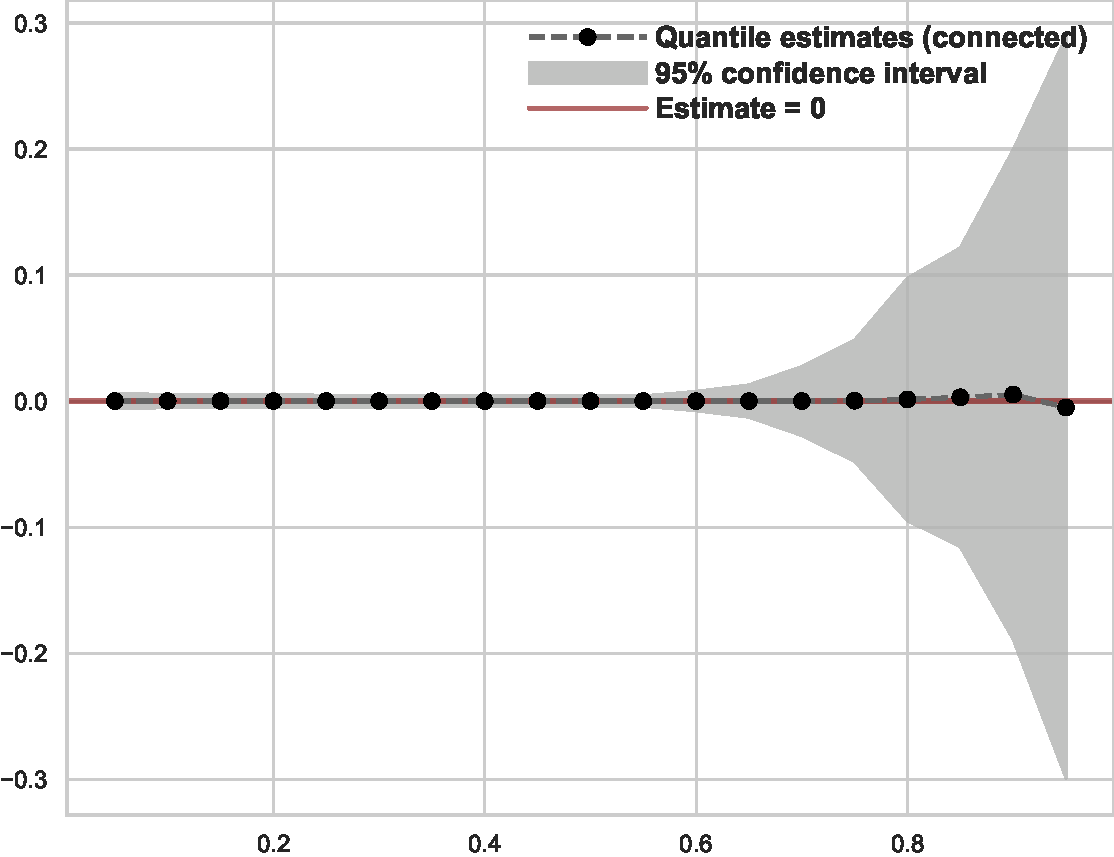
\includegraphics[width=.55\linewidth]{../figs/quantile_reg_covariates_duration_adult.pdf}
	\caption*{\footnotesize \emph{Notes:} 
		Dependent variable is the number of hours individuals in our sample spent on pornographic sites.
		Each point indicates the difference between Republicans and Democrats and corresponds to a quantile regression at the quantile indicated by the x-axis.
		Covariates included on the right-hand side are: gender (Female/Male), race (White/Black/Hispanic/Asian/Others), education level (no HS/HS graduate/some college/college graduate), age and its quadratic, and region (NE/MW/S/W).
		95\% confidence intervals constructed from standard errors.
		See \cref{fig:quantile_regression_duration} for the same plot without covariates.
	}
	\label{fig:quantile_regression_duration_covariates}
\end{figure}

%================================================================
% Fig of quantile regression estimates
% Percentage Time Spent on Adult Sites by Party (with covariates) 
%================================================================
\begin{figure}[ht]
	\centering
	\caption{Quantile Estimates--Percentage of Time Spent on Pornographic Sites by Party (with covariates)}
	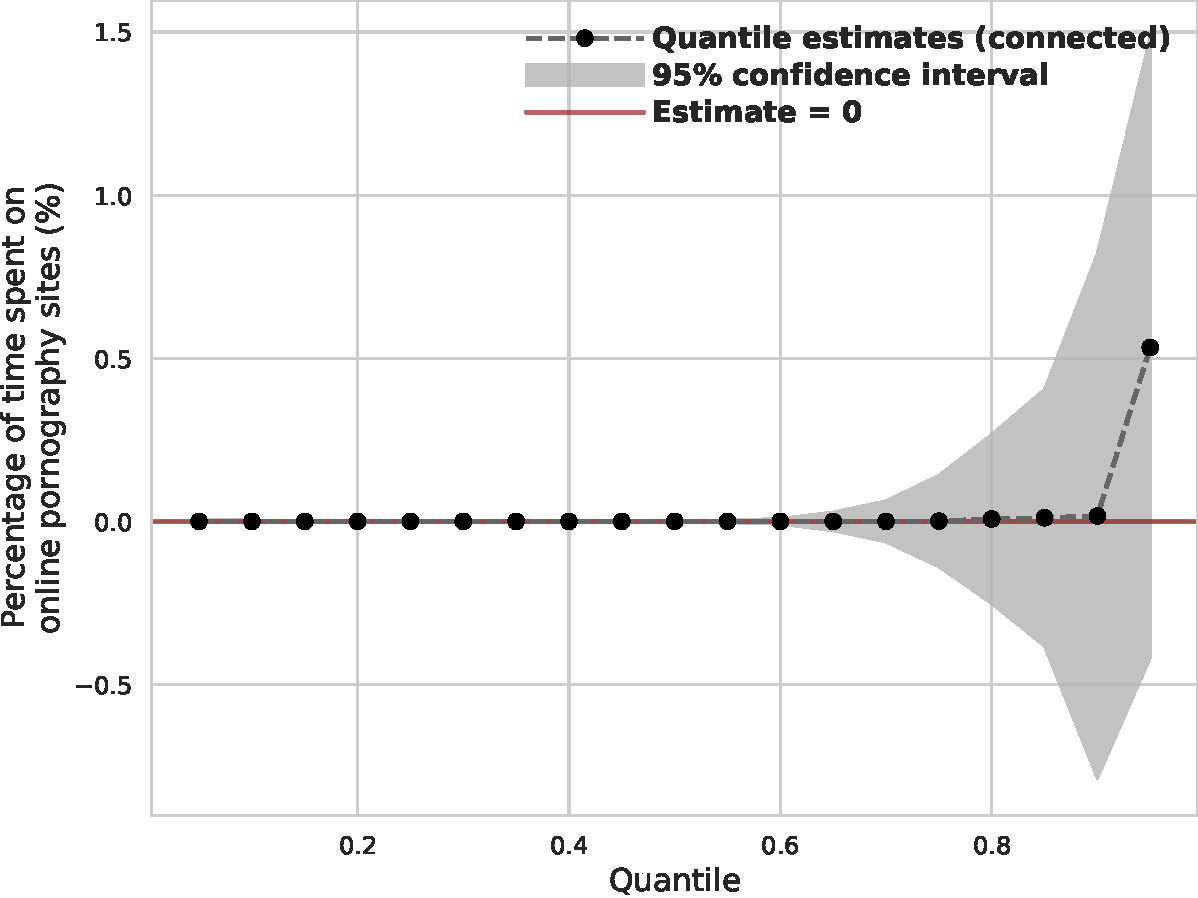
\includegraphics[width=.55\linewidth]{../figs/quantile_reg_covariates_proportion_duration_adult.pdf}
	\caption*{\footnotesize \emph{Notes:} 
		Dependent variable is the percentage of time individuals in our sample spent on pornographic sites.
		Each point indicates the difference between Republicans and Democrats and corresponds to a quantile regression at the quantile indicated by the x-axis.
		Covariates included on the right-hand side are: gender (Female/Male), race (White/Black/Hispanic/Asian/Others), education level (no HS/HS graduate/some college/college graduate), age and its quadratic, and region (NE/MW/S/W).
		95\% confidence intervals constructed from standard errors.
		See \cref{fig:quantile_regression_prop_duration} for the same plot without covariates.
	}
	\label{fig:quantile_regression_prop_duration_covariates}
\end{figure}
\clearpage

\FloatBarrier
%===============================================================================
% Consequence of Using Alternate Ways of Measuring Pornography and Alternative Analyses on Time Spent on Pornography
%===============================================================================
\section{Alternate Ways of Measuring Pornography}
\label{si:alternate_ways}
\clearpage

\section{Consumption of Pornography Among Independents}

\FloatBarrier
\section{Alternate Measures}
%============================================================================
% Figure of porn consumption by party
% Y-axis = proportion of individuals that ever consumed porn in sample period
%============================================================================

\subsection{Proportion of Partisans Who Consumed Any Pornography}
\begin{figure}
	\centering
	\caption{Pornography Consumption by Party}
	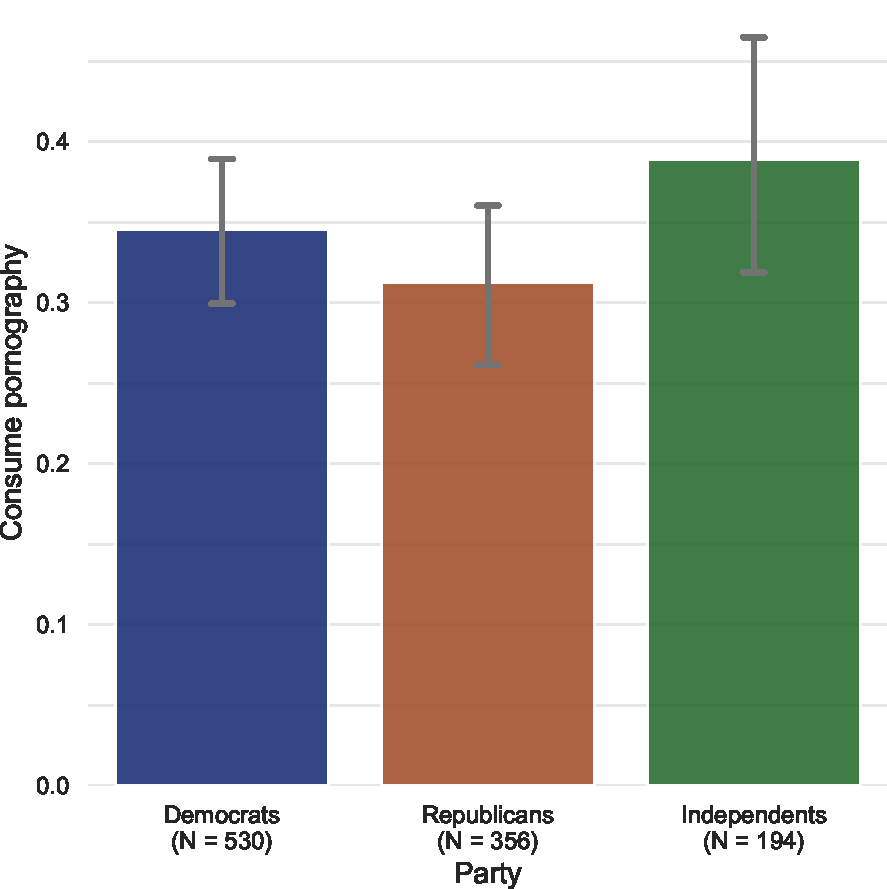
\includegraphics[width=.5\textwidth]{../figs/consume_porn_yes_no.pdf}
	\caption*{\footnotesize \emph{Notes:} 
		Figure shows proportion of individuals in the sample who ever consumed pornography in the sample period by party.
		Capped vertical bars are 95\% confidence intervals from bootstrapped standard errors (n = 1,000).
	}
	\label{fig:consume_porn_yes_no}
\end{figure}
\clearpage

\FloatBarrier
%===============================================================================
%===============================================================================
% Analogous results for visits to adult sites
%===============================================================================
%===============================================================================
\subsection{Analyses of Visits}
\label{si:visits}
%=================================================
% Figure for Distribution of visits to adult sites
%=================================================
\begin{figure}[ht]
	\centering
	\caption{Distribution of Traffic to Pornography Online}
	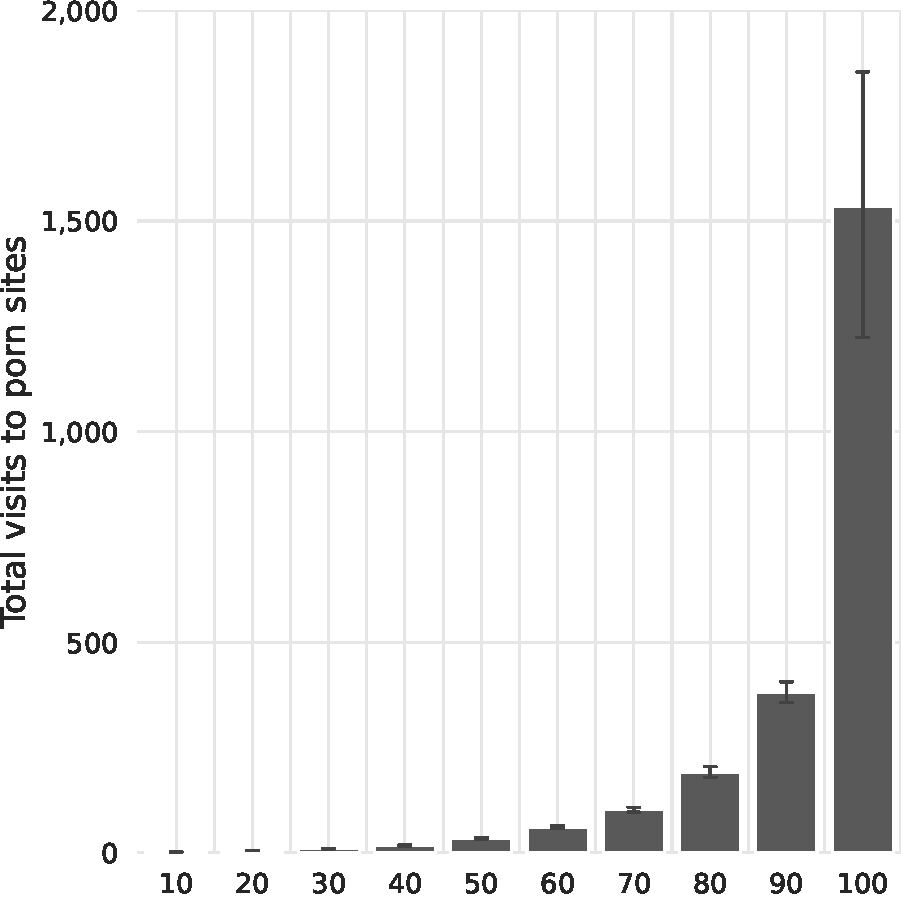
\includegraphics[width=.5\linewidth]{../figs/distribution_visits_to_adultsites.pdf}
	\caption*{\footnotesize \emph{Notes:} 
		Figure shows the number of visits to pornography sites by individuals who consumed pornography in the sample period.
		Individuals are split into deciles with each bin containing approximately the same number of individuals.
		Height of bars indicate mean of each bin.
		Capped vertical bars are 95\% confidence intervals.
		%See \cref{tab:distribution_visits} for the more tabulated values.
	}
	\label{fig:distribution_visits}
\end{figure}




%===============================================================
% Figure for Distribution of proportion of visits to adult sites
%===============================================================
\begin{figure}
	\centering
	\caption{Percentage of Traffic to Pornography Online}
	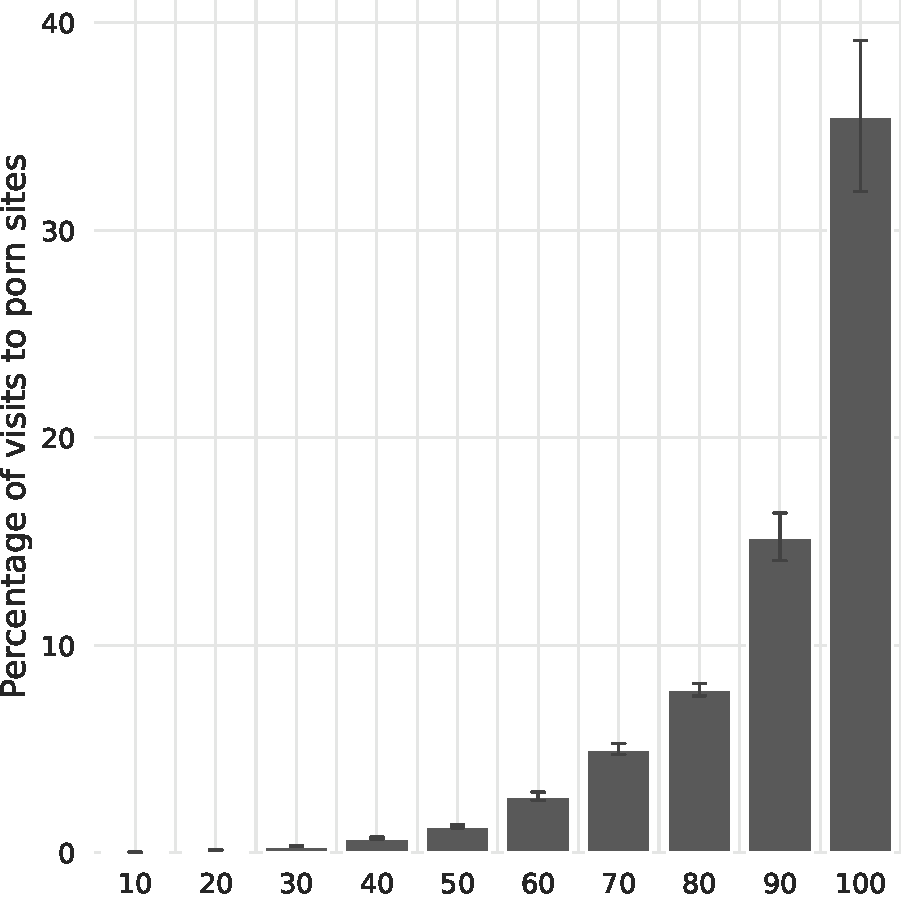
\includegraphics[width=.5\linewidth]{../figs/distribution_proportion_visits_to_adultsites.pdf}
	\caption*{\footnotesize \emph{Notes:} 
		Figure shows the proportion of visits to pornography sites by individuals who consumed pornography in the sample period.
		Individuals are split into deciles with each bin containing approximately the same number of individuals.
		Height of bars indicate mean of each bin.
		Capped vertical bars are 95\% confidence intervals.
		%See \cref{tab:distribution_prop_visits} for the more tabulated values.
	}
	\label{fig:distribution_prop_visits}
\end{figure}

%=======================
% Quantile regressions
% Traffic to adult sites
%=======================
\begin{figure}
	\centering
	\caption{Quantile Estimates--Traffic to Pornography Sites by Party}
	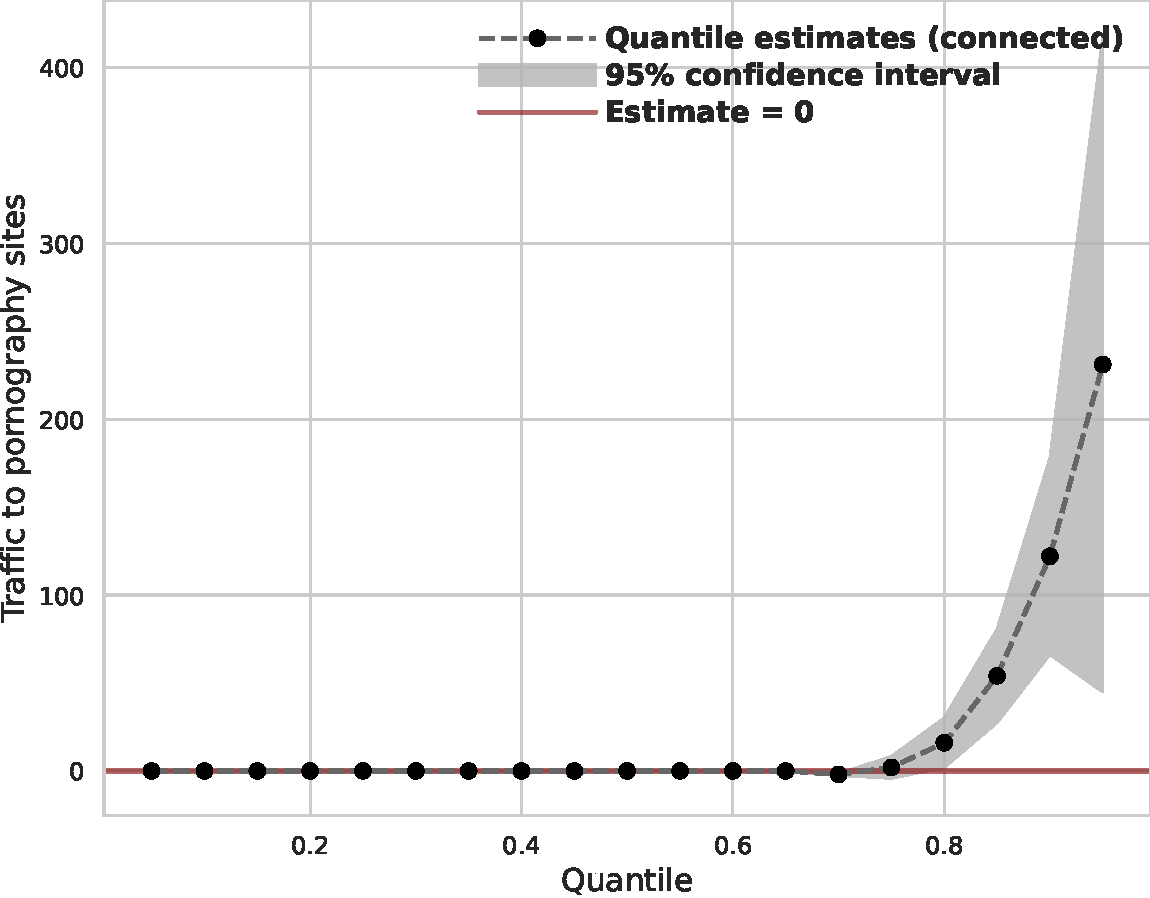
\includegraphics[width=.6\linewidth]{../figs/quantile_reg_visits_adult.pdf}
	\caption*{\footnotesize \emph{Notes:} 
		Dependent variable is the number of visits to pornographic sites by individuals in our sample.
		Each point indicates the difference between Republicans and Democrats and corresponds to a quantile regression at the quantile indicated by the x-axis.
		95\% confidence intervals constructed from standard errors.
		%See \cref{fig:quantile_regression_visits_covariates} for the same plot controlling for individual characteristics.
	}
	\label{fig:quantile_regression_visits}
\end{figure}

%=====================================
% Quantile regressions
% Proportion of traffic to adult sites
%=====================================
\begin{figure}
	\centering
	\caption{Quantile Estimates--Percentage of Traffic to Pornographic Sites by Party}
	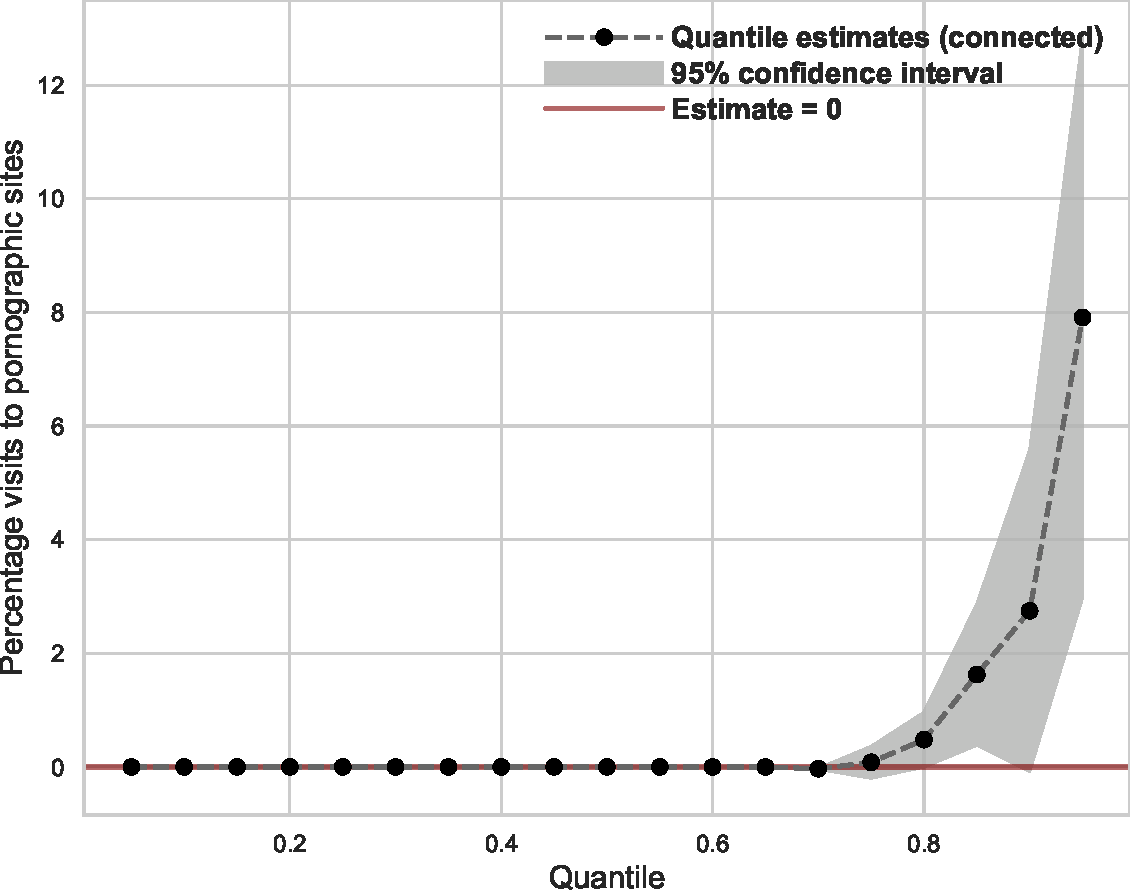
\includegraphics[width=.6\linewidth]{../figs/quantile_reg_proportion_visits_adult.pdf}
	\caption*{\footnotesize \emph{Notes:} 
		Dependent variable is the percentage of traffic to pornographic sites by individuals in our sample.
		Each point indicates the difference between Republicans and Democrats and corresponds to a quantile regression at the quantile indicated by the x-axis.
		95\% confidence intervals constructed from standard errors.
		%See \cref{fig:quantile_regression_prop_visits_covariates} for the same plot controlling for individual characteristics.
	}
	\label{fig:quantile_regression_prop_visits}
\end{figure}


%==================================================
% Fig of quantile regression estimates
% Traffic to Adult Sites by Party (with covariates) 
%==================================================
\begin{figure}
	\centering
	\caption{Quantile Estimates--Traffic to Pornographic Sites by Party (with covariates)}
	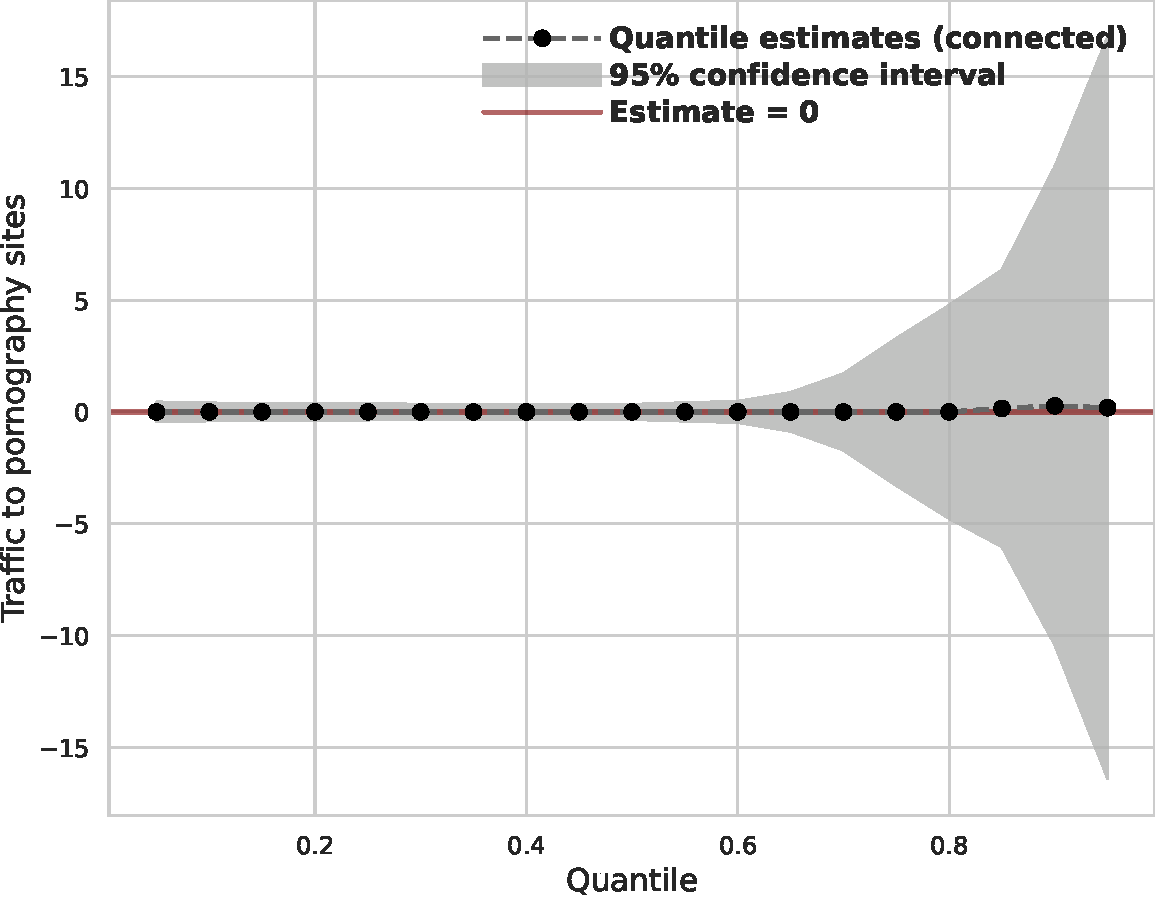
\includegraphics[width=.55\linewidth]{../figs/quantile_reg_covariates_visits_adult.pdf}
	\caption*{\footnotesize \emph{Notes:} 
		Dependent variable is the number of visits to pornographic sites by individuals in our sample.
		Each point indicates the difference between Republicans and Democrats and corresponds to a quantile regression at the quantile indicated by the x-axis.
		Covariates included on the right-hand side are: gender (Female/Male), race (White/Black/Hispanic/Asian/Others), education level (no HS/HS graduate/some college/college graduate), age and its quadratic, and region (NE/MW/S/W).
		95\% confidence intervals constructed from standard errors.
		%See \cref{fig:quantile_regression_visits} for the same plot without covariates.
	}
	\label{fig:quantile_regression_visits_covariates}
\end{figure}



%=============================================================
% Fig of quantile regression estimates
% Percentage Traffic to Adult Sites by Party (with covariates) 
%=============================================================
\begin{figure}
	\centering
	\caption{Quantile Estimates--Percentage of Traffic to Pornographic Sites by Party (with covariates)}
	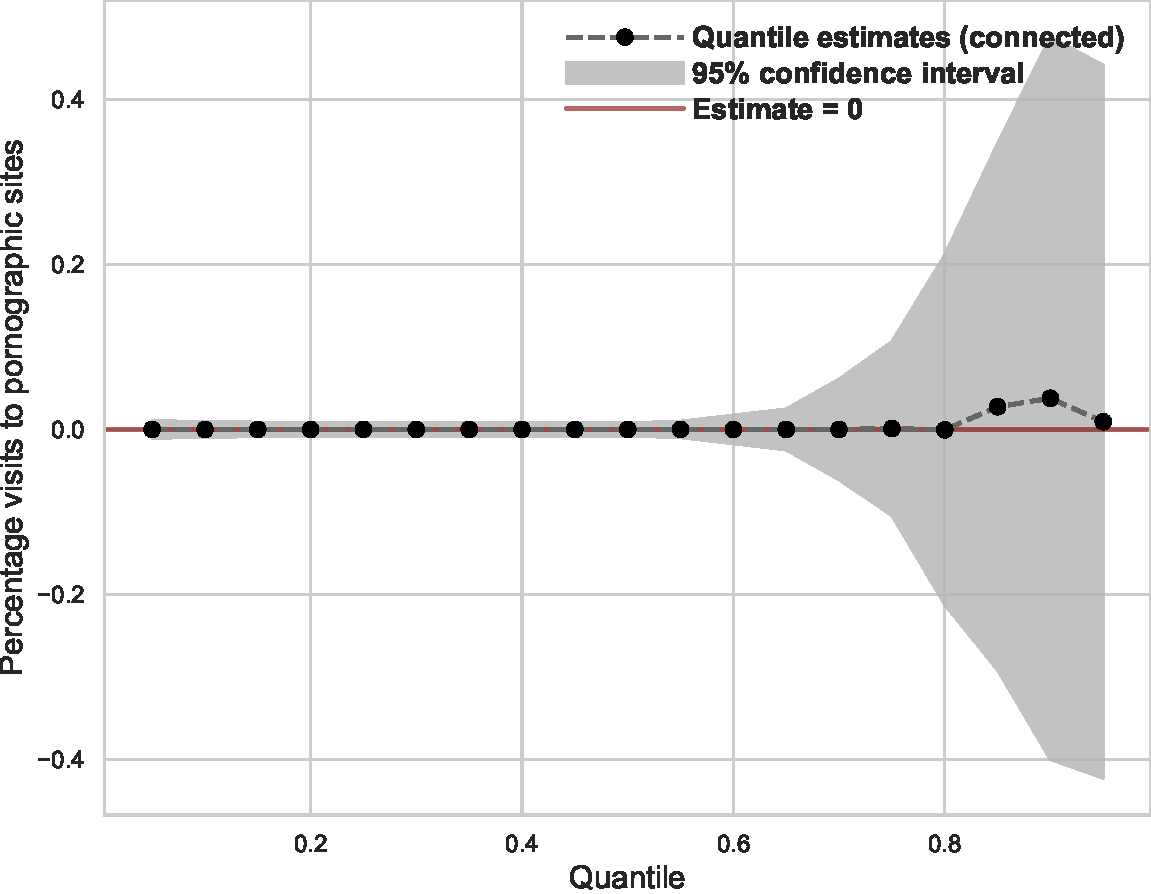
\includegraphics[width=.55\linewidth]{../figs/quantile_reg_covariates_proportion_visits_adult.pdf}
	\caption*{\footnotesize \emph{Notes:} 
		Dependent variable is the percentage of traffic to pornographic sites by individuals in our sample.
		Each point indicates the difference between Republicans and Democrats and corresponds to a quantile regression at the quantile indicated by the x-axis.
		Covariates included on the right-hand side are: gender (Female/Male), race (White/Black/Hispanic/Asian/Others), education level (no HS/HS graduate/some college/college graduate), age and its quadratic, and region (NE/MW/S/W).
		95\% confidence intervals constructed from standard errors.
		%See \cref{fig:quantile_regression_prop_visits} for the same plot without covariates.
	}
	\label{fig:quantile_regression_prop_visits_covariates}
\end{figure}




\end{document}
